\subsection{Encoding}
\label{sec:math_encoding}

Some elliptic curve based cryptosystems (such as the adapted ElGamal in Section \ref{sec:math_encryption}) are constructed to encrypt points on a curve. To make
this useful an original string message must be encoded as a point. The encoding must be reversible.

It is trivial to map a message string to the correct numberspace as both strings and numbers have binary representations. The number is then
simply found by converting a string to its binary representation and interpreting this as an integer. Using the ASCII character set the string
\verb+"A"+ is mapped to the number \verb+65+.

\begin{verbatim}
    string_to_binary "A" -> 1000001
    binary_to_integer 1000001 ->  65
\end{verbatim}

Koblitz is attributed with an algorithm that maps a message \(m\), represented as an integer in \(\mathbb{Z}_p\), to a point on the curve of the
simple Weierstrass form \(y^2 = x^3 + ax + b \text{ mod } p\).\cite{MappingAMessage}

An integer K is selected such that \((M + 1)K < p\), and this is used to compute
a candidate x-coordinate for the point, \(x_j = MK + j \text{ mod } p\). To verify the validity of the candidate, a check is performed: \(x_j\)
is a valid x-coordinate for a point on the curve if \(z_j = x_j^3 + ax_j + b\) has a square root. If the candidate is valid, the message \(m\)
can be mapped to a point \(M\) on the curve:

\begin{equation}
	M = (x_j, y_j) \text{, where } y_j = \sqrt{z_j} \text{ mod } p
\end{equation}

If no square root exists for \(z_j\) for all \(j\), \(j = 0 \text{ to } K-1\), then it is not possible to map the message to a point. In other
words, the method is probablistic and it is possible that a message cannot be encoded.

To find the original message from a point again, a simple calculcation is performed:

\begin{equation}
	m = {\lfloor {x \over K} \rfloor}
\end{equation}

The flooring of \(x \over K\) ensures that any \(j\) added to \(MK\) has no effect.\cite{MappingAMessage}

As the numberspace the messages must be mapped to is limited by the size of the prime field \(\mathbb{F}_p\) over which the curve is defined, so is the
length of the message. The numeric value of a string can be no greater than \(p\).

\paragraph{Picking the value K}

The selection of value \(K\) has implications on both the probability that a message can be mapped, and the performance of the encoding algoirthm.
The probability of successful encoding is described as \(P_{success} \geq 1 - {1 \over {2^K}}\): the larger the value of \(K\), the greater the probability,
as shown in Figure \ref{fig:probability}. With \(K\) greater than 6, no discernible change in probability occurs.\cite{MappingAMessage}

\begin{figure}[htb]
	\centering
	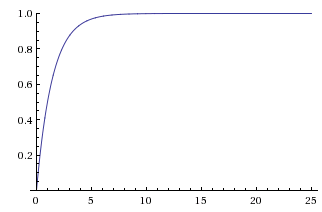
\includegraphics[width=0.6\textwidth]{maths/encoding-probability}
	\caption{Minimum probability of successful encoding, depending on size of K.}
	\label{fig:probability}
\end{figure}

The performance of the mapping depends on three calculations: (1) the multiplication \(MK\); (2) the calculation of \(z_j\), specifically
performing the calculations \(x_j^3\) and \(ax_j\); and (3) the computation of a potential root \(\sqrt{z_j}\). While the first calculation (1)
is performed only once, the last two (2,3) are repeated until a root is found, or all possible values have been tried.

Multiplication is a heavy operation, and picking a smaller value of \(K\) limits both the load of each multiplications (as they are performed with
smaller numbers), and the number of multiplications (as the range of \(j\)s used is limited by \(K - 1\)). So while it is easy to find the greatest
possible value \(K_greatest = {\lfloor { p \over {MK} }\rfloor}\), yielding the highest probability of success, this is not necessarily desirable.
Picking \(K = 7\) gives a probability of success \(P_{success} \geq 0.993\) -- high enough for our purposes.